\documentclass[a4paper]{article}
\usepackage{graphicx}
\usepackage[hidelinks]{hyperref}
\usepackage{xcolor}
\usepackage{url}
\usepackage{outlines}
\usepackage{listings}
\usepackage{fontspec}
\usepackage{parskip}
\usepackage[dvipsnames]{xcolor}
\usepackage{minted}
\lstset{basicstyle=\ttfamily,
	showstringspaces=false,
	commentstyle=\color{blue},
	keywordstyle=\color{RubineRed}
}
\lstset{emph={
	COPY,EXPOSE,RUN,FROM,CMD,nc,tcp,udp,http,docker},emphstyle=\color{purple}
}
\lstdefinestyle{yaml}{
     basicstyle=\color{RubineRed}\ttfamily,
     rulecolor=\color{blue},
     string=[s]{'}{'},
     stringstyle=\color{black},
     comment=[l]{\#},
     commentstyle=\color{blue},
     morecomment=[l]{-}
 }
\newcommand{\abc}{\hfill \break}
\usepackage{fancyhdr}
\usepackage{geometry}
\geometry{
	a4paper,
	total={170mm,257mm},
	left=20mm,
	top=20mm,
	bottom=39mm,
}

\setlength{\headheight}{82.70538pt}

\fancypagestyle{oida}{
	\fancyhf{}
	\fancyhead[L]{\fontsize{7.5}{7.5}htl donaustadt\\ Donaustadtstraße 45\\
		1220 Wien\\~\\ Abteilung: Informationstechnologie\\ 
	Schwerpunkt: Netzwerktechnik}
	\fancyhead[R]{
\includegraphics[scale=0.45]{images/logo.png}}

	\fancyfoot[L]{\today}
	\fancyfoot[C]{\jobname}
	\fancyfoot[R]{Page: \thepage}
}

\begin{document}
\bibliographystyle{IEEEtran}
\pagestyle{oida}
\section*{Exercise 6: GNU/Linux - Securing active components}
\par\noindent\rule{\textwidth}{0.4pt}

Laboratory protocol
\begin{figure}[h]
	
\includegraphics[scale=0.3]{images/mika.jpeg}
	\caption{Grouplogo}
\end{figure}

\vspace*{\fill}
Subject:	ITSI

Class:	3AHITN

Name:	Stefan Fürst, Marcel Raichle

Gruppenname/Nummer: Dumm und Dümmer/7

Supervisor: 	SPAC, ZIVK

Exercise dates:	3.1.2025, 4.1.2025

Submission date: 4.1.2025


\newpage
\tableofcontents

\newpage

\section{Task definition}



\section{Summary}

\newpage

\section{Complete network topology of the exercise}

\begin{figure}[h]
	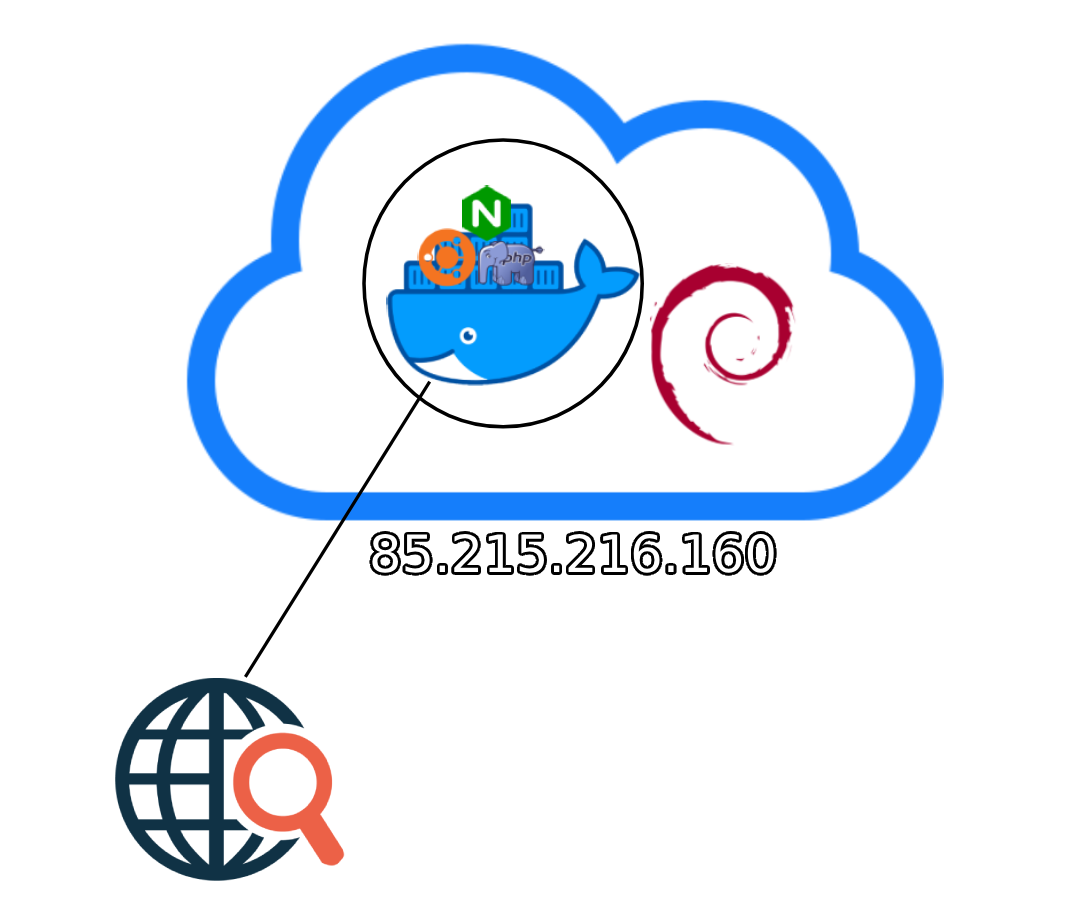
\includegraphics[scale=0.3]{images/topology.png}
	\centering
	\caption{Network topology of this exercise}
\end{figure}

\newpage

\section{Exercise Execution}

\subsection{Preparation}
The requirements for this exercise are a headless Linux server with hardened SSH, which only allows connections via key pairs. However, I removed the OTP authentication added in the last exercise, as it was overkill for this use case and became a burden to use.
\begin{figure}[h]
	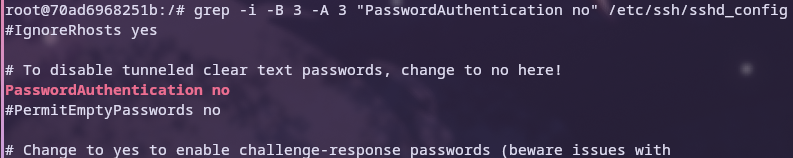
\includegraphics[scale=0.26]{images/sshnopw.png}
	\centering
	\caption{Password authentication disabled}
\end{figure} 
\subsection {Testing the SSH connectivity.}
\begin{figure}[h]
	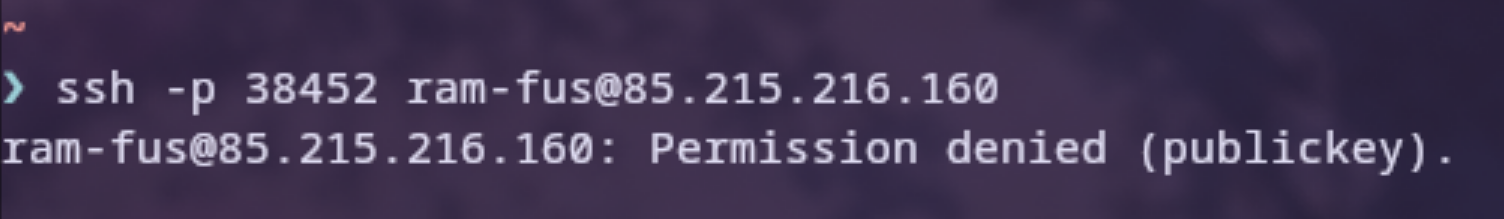
\includegraphics[scale=0.13]{images/nokey.png}
	\centering
	\caption{No SSH key available}
\end{figure}
\begin{figure}[!hbp]
	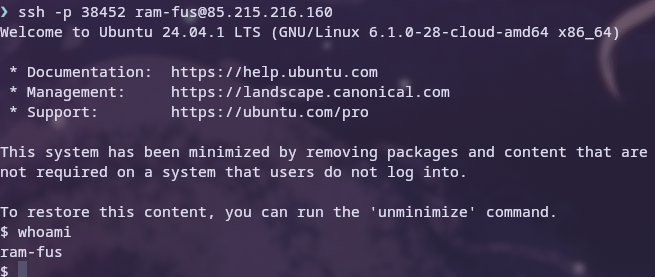
\includegraphics[scale=0.3]{images/yeskey.png}
	\centering
	\caption{ram-fus authenticating via SSH key}
\end{figure}

\begin{figure}[!htbp]
	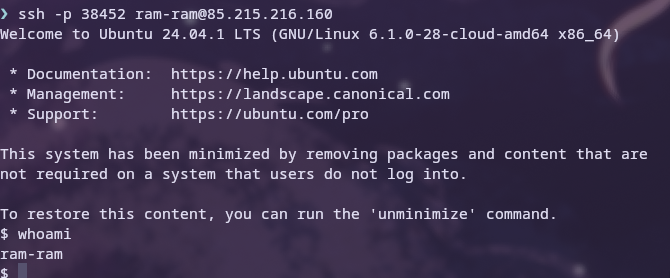
\includegraphics[scale=0.3]{images/yeskey2.png}
	\centering
	\caption{ram-ram authenticating via SSH key}
\end{figure}\newpage
\subsubsection{Changes to the Docker setup}
To improve the quality of life when working on this project, I switched from aliasing a long and hard-to-read run command to using Docker Compose, which allows you to define and run multi-container applications. Since it's in a YAML file, it is more readable and easier to work with, even in this use case where I only have one container.\cite{Docker-Compose}
\begin{lstlisting}[language=bash]
services:
    #setting the name image and restart policy
    webserver:
        container_name: itsi
        image: itsi:latest
        restart: no
    #setting exposed ports
    ports:
        - "38452:38452"
        - "80:80"
        - "443:443"
\end{lstlisting}
To still utilize my alias script, I changed every instance of \texttt{docker run} to \texttt{docker compose up -d}, \abc and \texttt{docker stop itsi \&\& docker rm itsi} to\texttt{docker compose down}.
\begin{lstlisting}[language=bash]
#!/bin/bash
alias relaunch="sh -c 'docker stop itsi && docker rm itsi &&\
		       docker buildx build -t itsi:latest . &&\
		       docker compose up -d && docker exec -it itsi /bin/bash'"
alias rebuild="sh -c 'docker buildx build -t itsi:latest . &&\
                      docker compose up -d && docker exec -it itsi /bin/bash'"
alias stop="sh -c 'docker compose down'"
\end{lstlisting}
Furthermore, instead of having to upload my container every time I rebuild, I added these three lines to copy the \texttt{authorized\_keys} file with the devices I use to the container, so that every time I relaunch, I can just immediately SSH into it.
\begin{lstlisting}[language=bash]
COPY ./mapped-files/authorized_keys /root/.ssh/authorized_keys
COPY ./mapped-files/authorized_keys /home/ram-fus/.ssh/authorized_keys
COPY ./mapped-files/authorized_keys /home/ram-ram/.ssh/authorized_keys
\end{lstlisting}
Lastly, the line in the Dockerfile that specifies the exposed ports is edited to expose ports 80 and 443, as they will be required for this exercise.
\begin{lstlisting}[language=bash]
EXPOSE 38452 80 443
\end{lstlisting}
\newpage
\subsection{Installing an active component}

Now, it's required to install a web server. I chose Nginx because I am most familiar with it, and due to its high performance and simplicity of use.\abc
It’s installed and run by adding these lines to the Dockerfile and including \texttt{service nginx start} on the last line.
\begin{lstlisting}[language=bash]
...
RUN apt install -y nginx
...
CMD service ssh start && service nginx start && tail -F /dev/null
\end{lstlisting}
After modifying the Dockerfile, rebuilding, and redeploying, if we now open the web browser and go to the server's IP, we see the following.
\begin{figure}[h]
	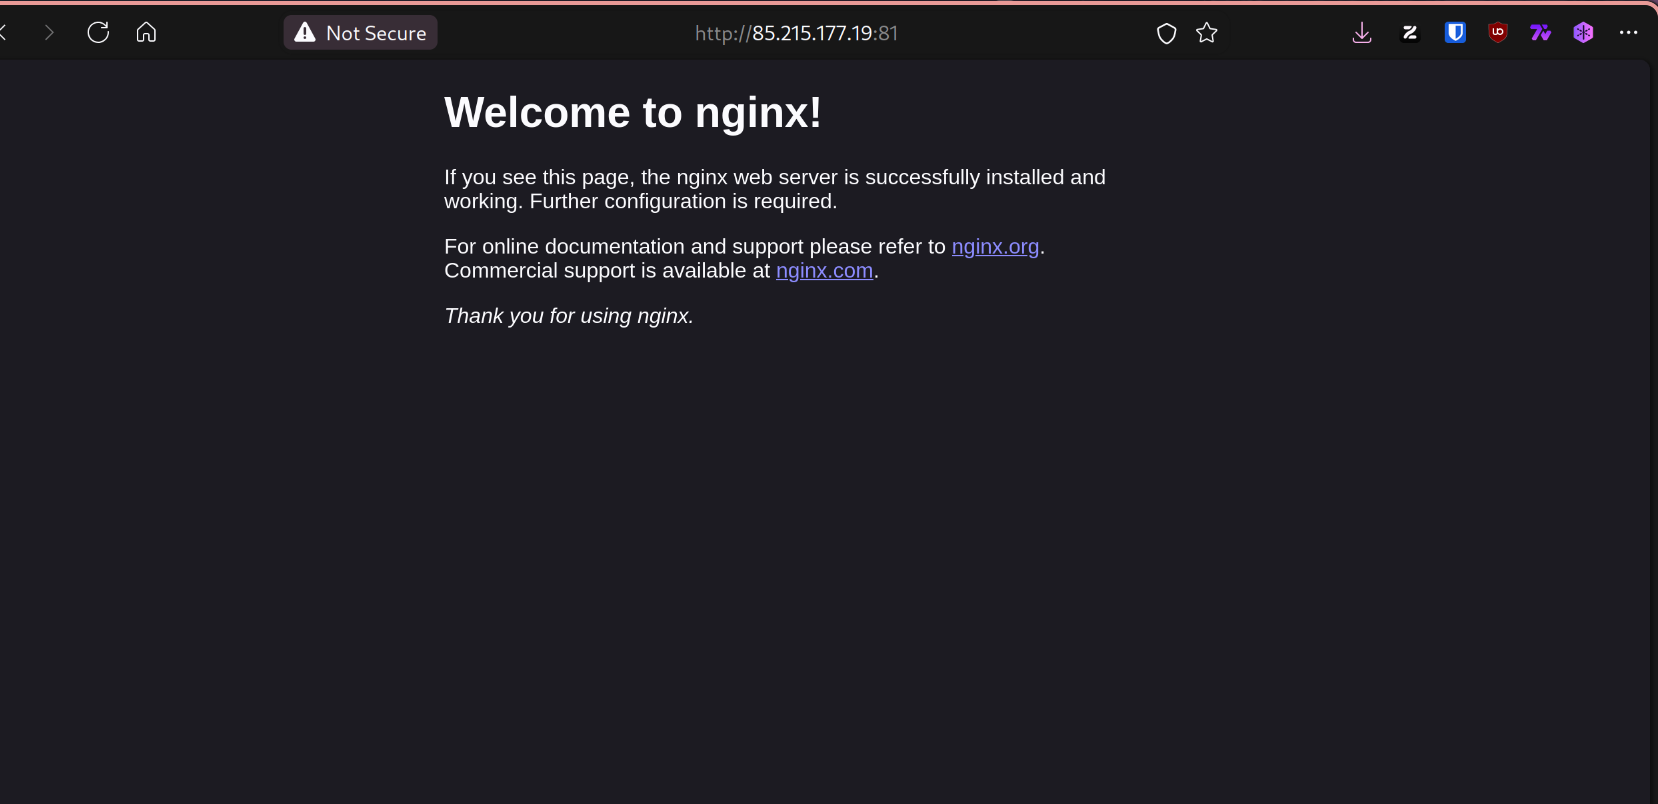
\includegraphics[scale=0.2]{images/nginx.png}
	\centering
	\caption{Default nginx site}
\end{figure}\footnote{The IP and port are different since, initially, I used a VPS that already had a web server running, so I had to change the port. After that, I switched to a new VPS, which will be used for the rest of the exercise.}\abc
The HTML site displayed is located at \texttt{/var/www/html/index.nginx-debian.html}.
Additionally, I replaced the \texttt{/var/www/html} directory with \texttt{/var/www/metyr.xyz}, in which I have the following file structure:
\begin{lstlisting}[language=bash]
`-- html
   |-- private
   |   `-- private.php
    `-- public
        `-- index.php
\end{lstlisting}
These two directories are mapped onto the Docker container in the \texttt{docker-compose.yml} file, as shown below. Since they are mapped, every time the files are changed on the host, the changes carry over to the container, allowing for an easy and fast development workflow without the need to exec into the container or copy the files when creating the image.
Nginx won't serve those PHP files without further configuration, which is explained in the next section.
\begin{lstlisting}[language=bash]
volumes:
    - ./mapped-files/public:/var/www/html/public:rw
    - ./mapped-files/private:/var/www/html/private:rw
\end{lstlisting}
Additionally, I edited the Dockerfile to delete the default Nginx configuration file, located at \texttt{/etc/nginx/sites-enabled/default}, a symlink to the file \texttt{/etc/nginx/sites-available/default.conf}, and replaced it with one matching my domain name for better readability.\newpage
\begin{lstlisting}[language=bash]
RUN rm -rf /var/www/html/
RUN mkdir -p /var/www/metyr.xyz/html
RUN rm /etc/nginx/sites-available/default
RUN rm /etc/nginx/sites-enabled/default
#copying the configuration file to the container during the build process
COPY ./mapped-files/metyr.xyz /etc/nginx/sites-available/metyr.xyz
#symlinking the new configuration file to enable the site
RUN ln -s /etc/nginx/sites-available/metyr.xyz /etc/nginx/sites-enabled/metyr.xyz
\end{lstlisting}
\subsubsection{Setting up PHP-FPM with Nginx}
To give Nginx the ability to serve PHP files, the \texttt{php-fpm} (FastCGI Process Manager) package is required.
With this package installed, the following lines can be added to the server block in the Nginx configuration file.
\begin{lstlisting}[language=bash]
server{
	...
	#setting the location of the index file to serve
	index public/index.php;
	#location block, which matches requests for files ending with .php
	location ~ \.php$ {
		#include the fastcgi-php configuration file
		include snippets/fastcgi-php.conf;
		#passing the requets to the FastCGI server on set socket
		fastcgi_pass unix:/run/php/php8.3-fpm.sock;
	}
	...
}
\end{lstlisting}
Additionally, the \texttt{php-fpm} service has to be started, so the default command of the container is edited.
\begin{lstlisting}[language=bash]
CMD service ssh start && service nginx start && service php8.3-fpm start\
    && tail -F /dev/null
\end{lstlisting}
If we now rebuild the container, deploy it, and go to the IP address of the server in the browser, we can see the PHP page displayed.
The site has a public part, located at \texttt{public/index.php}, and a private part, located at \texttt{private/private.php}. The private part contains the number and members of my group, along with an AI-generated image, which is why it requires authentication to access. This will be explained in the next section.\abc
\begin{figure}[!htbp]
	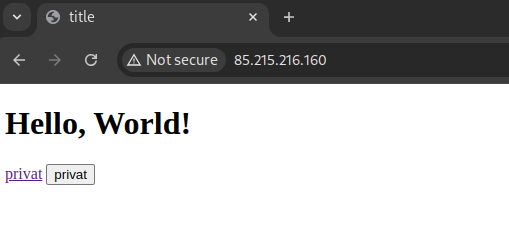
\includegraphics[scale=0.45]{images/indexphp.png}
	\centering
	\caption{Viewing the index of the website}
\end{figure}
\begin{figure}[!htbp]
	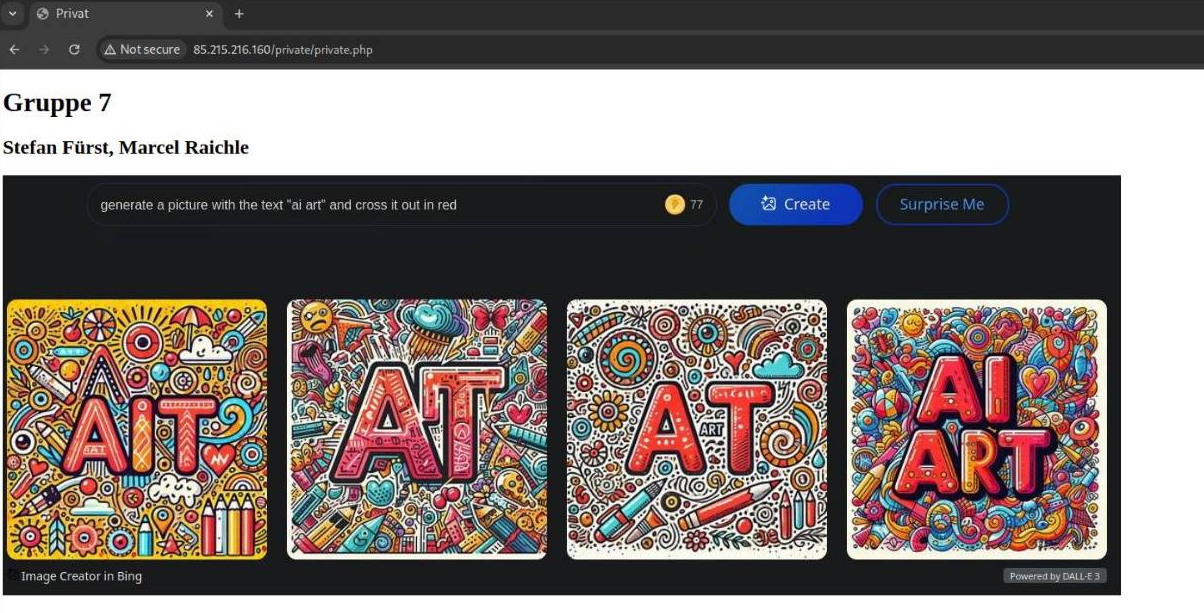
\includegraphics[scale=0.2]{images/privatphp.png}
	\centering
	\caption{Viewing the private part of the website}
\end{figure}\abc\newpage
\subsection{Securing Nginx with Basic Authentication}

\subsection{Configuring HTTPS with Self-Signed Certificates}

\subsection{Adding a Domain}

\newpage
\section{References}
\bibliography{IEEEabrv,quellen}
\newpage
\section{List of figures}

\listoffigures

\end{document}
